%\documentclass[a4paper, 12pt]{scrreprt}

\documentclass[a4paper, 12pt]{scrartcl}
%usepackage[german]{babel}
\usepackage{microtype}
%\usepackage{amsmath}
%usepackage{color}
\usepackage[utf8]{inputenc}
\usepackage[T1]{fontenc}
\usepackage{wrapfig}
\usepackage{lipsum}% Dummy-Text
\usepackage{multicol}
\usepackage{alltt}
%%%%%%%%%%%%bis hierhin alle nötigen userpackage
\usepackage{tabularx}
\usepackage[utf8]{inputenc}
\usepackage{amsmath}
\usepackage{amsfonts}
\usepackage{amssymb}

%\usepackage{wrapfig}
\usepackage[ngerman]{babel}
\usepackage[left=25mm,top=25mm,right=25mm,bottom=25mm]{geometry}
%\usepackage{floatrow}
\setlength{\parindent}{0em}
\usepackage[font=footnotesize,labelfont=bf]{caption}
\numberwithin{figure}{section}
\numberwithin{table}{section}
\usepackage{subcaption}
\usepackage{float}
\usepackage{url}
%\usepackage{fancyhdr}
\usepackage{array}
\usepackage{geometry}
%\usepackage[nottoc,numbib]{tocbibind}
\usepackage[pdfpagelabels=true]{hyperref}
\usepackage[font=footnotesize,labelfont=bf]{caption}
\usepackage[T1]{fontenc}
\usepackage {palatino}
%\usepackage[numbers,super]{natbib}
%\usepackage{textcomp}
\usepackage[version=4]{mhchem}
\usepackage{subcaption}
\captionsetup{format=plain}
\usepackage[nomessages]{fp}
\usepackage{siunitx}
\sisetup{exponent-product = \cdot, output-product = \cdot}
\usepackage{hyperref}
\usepackage{longtable}
\newcolumntype{L}[1]{>{\raggedright\arraybackslash}p{#1}} % linksbündig mit Breitenangabe
\newcolumntype{C}[1]{>{\centering\arraybackslash}p{#1}} % zentriert mit Breitenangabe
\newcolumntype{R}[1]{>{\raggedleft\arraybackslash}p{#1}} % rechtsbündig mit Breitenangabe
\usepackage{booktabs}
\renewcommand*{\doublerulesep}{1ex}
\usepackage{graphicx}
\usepackage{chemformula}


\usepackage[backend=bibtex, style=chem-angew, backref=none, backrefstyle=all+]{biblatex}
\bibliography{Literatur.bib}
\defbibheading{head}{\section{Literatur}\label{sec:Lit}} 
\let\cite=\supercite
\begin{document}
\setlength\abovedisplayshortskip{20pt}
\setlength\belowdisplayshortskip{20pt}
\setlength\abovedisplayskip{20pt}
\setlength\belowdisplayskip{20pt}
\section {Anhang}
\begin{figure}[H]
	\centering	
	\begin{minipage}{1\textwidth}
		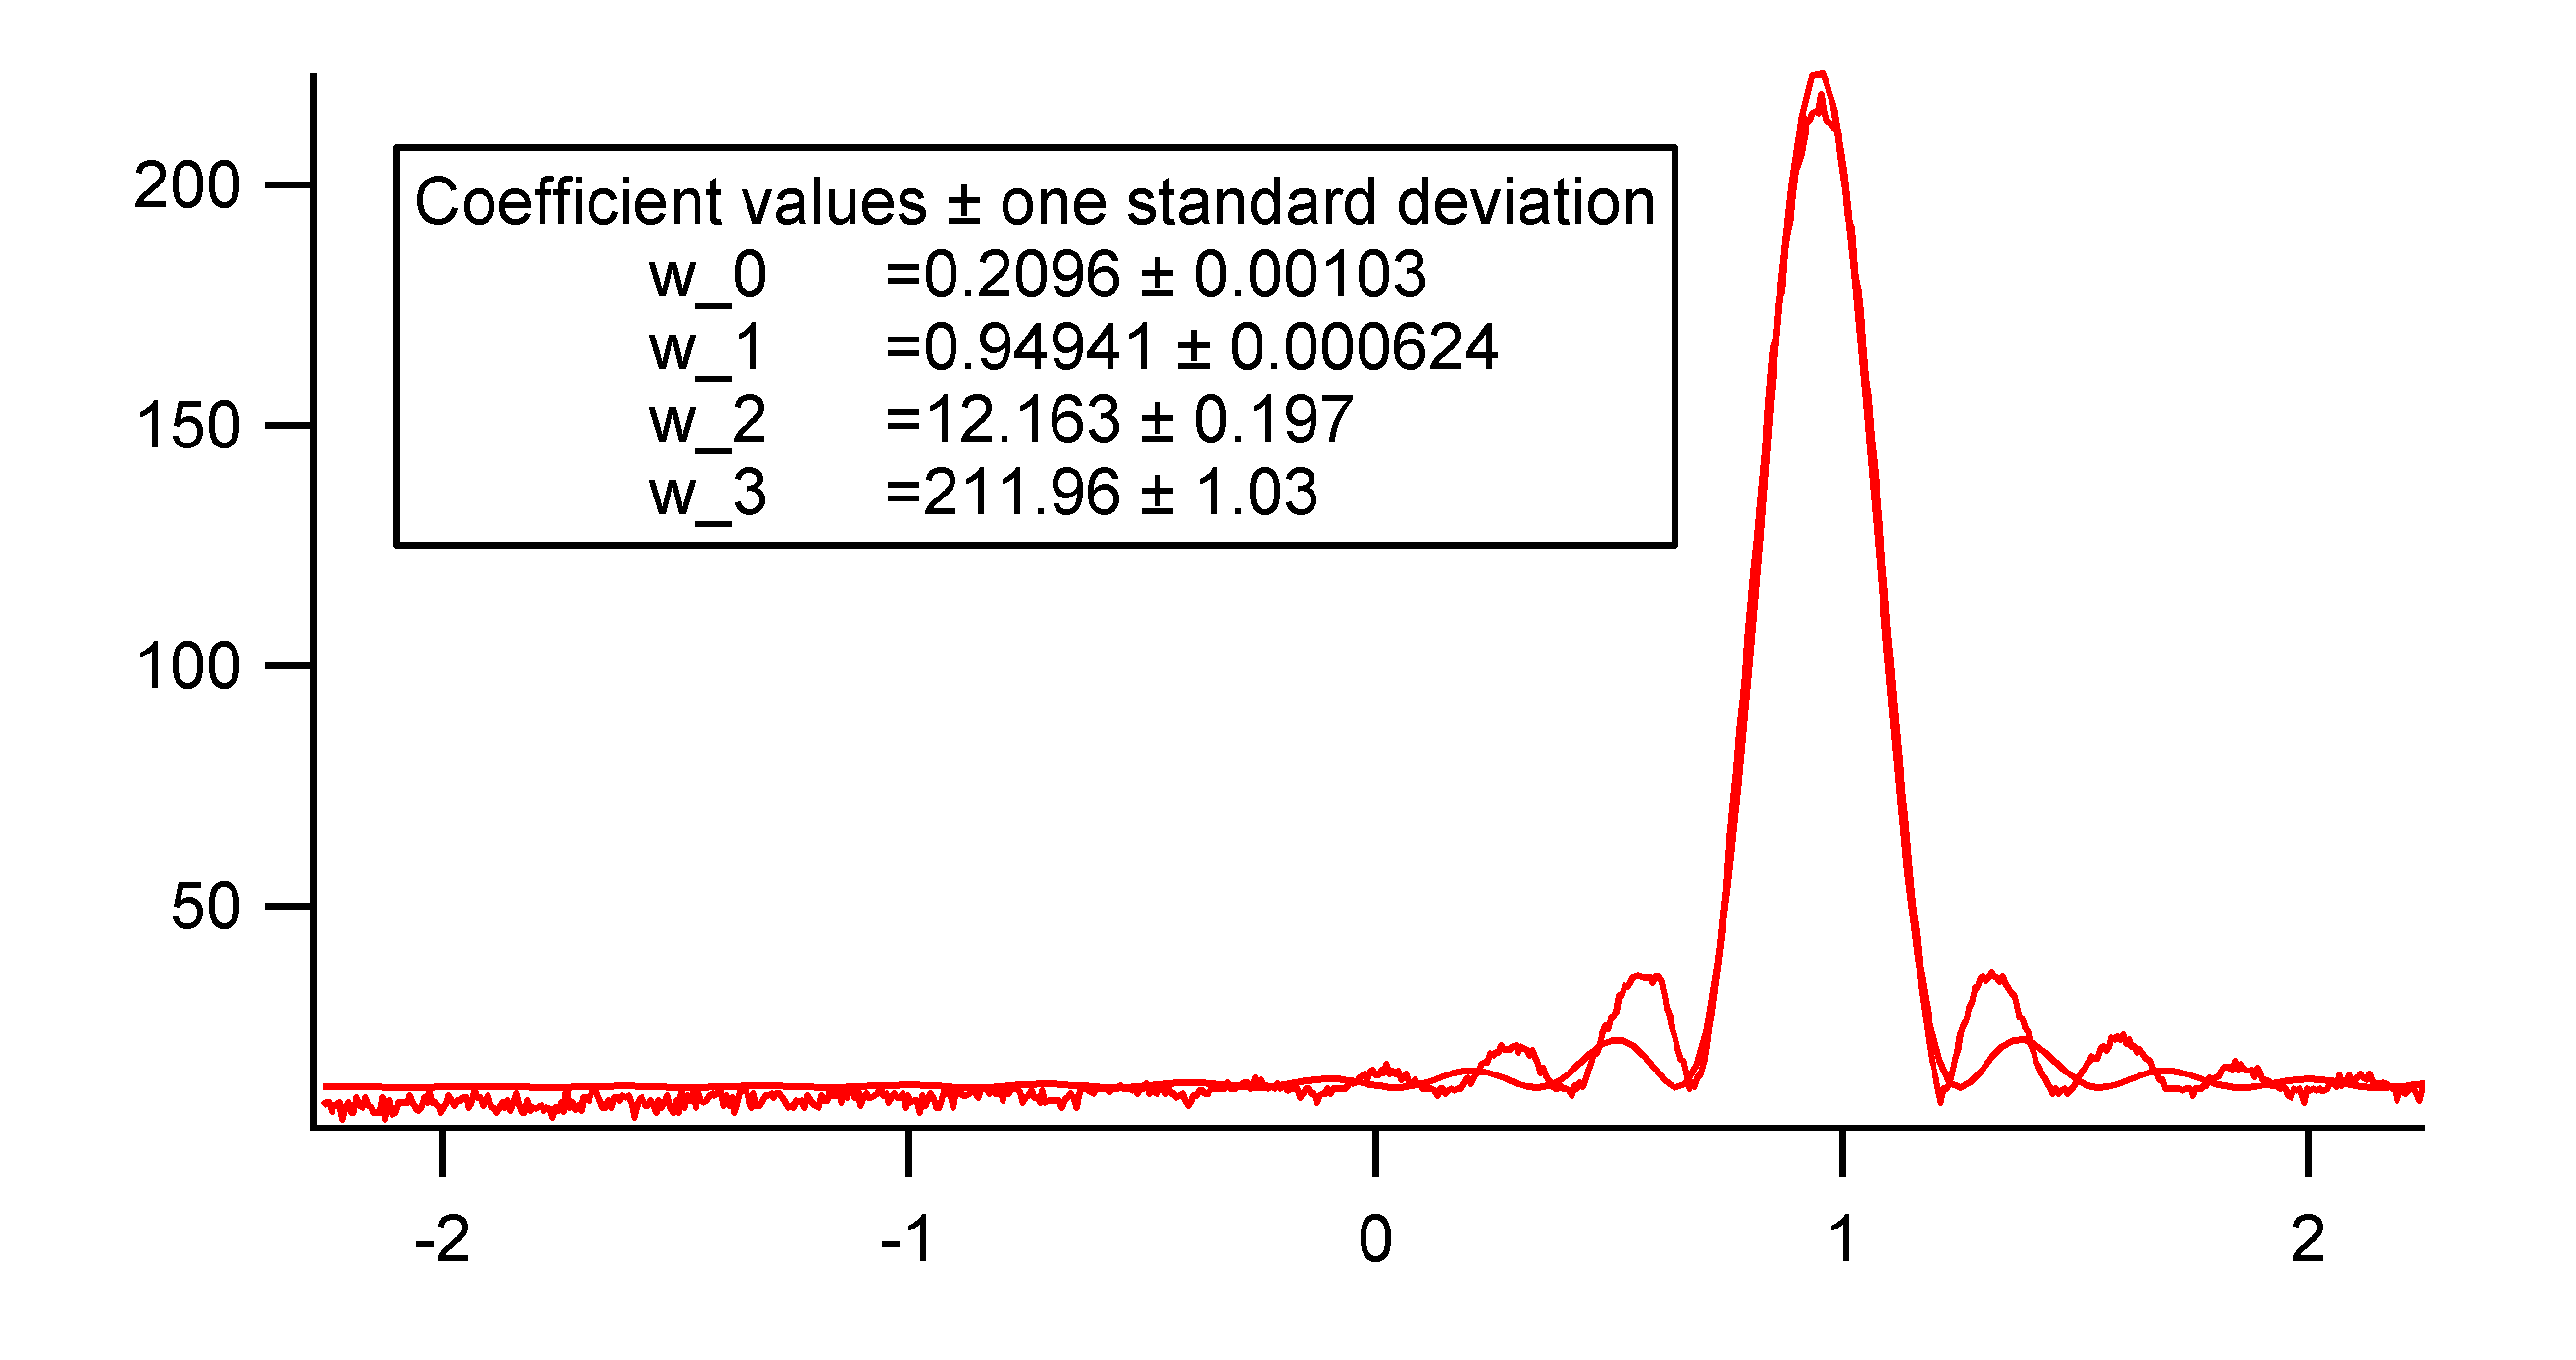
\includegraphics[width=\columnwidth]{180618/Graph1.png}
	\end{minipage}
	\caption{Beugungsmuster eines Helium-Neon-Lasers bei der Einstellung von $4~\mu m$. Der Querschnitt wurde mit Igor Pro ausgewählt und weiter analysiert }
	\label{HeNe_1}
\end{figure}
\begin{figure}[H]
	\centering	
	\begin{minipage}{1\textwidth}
		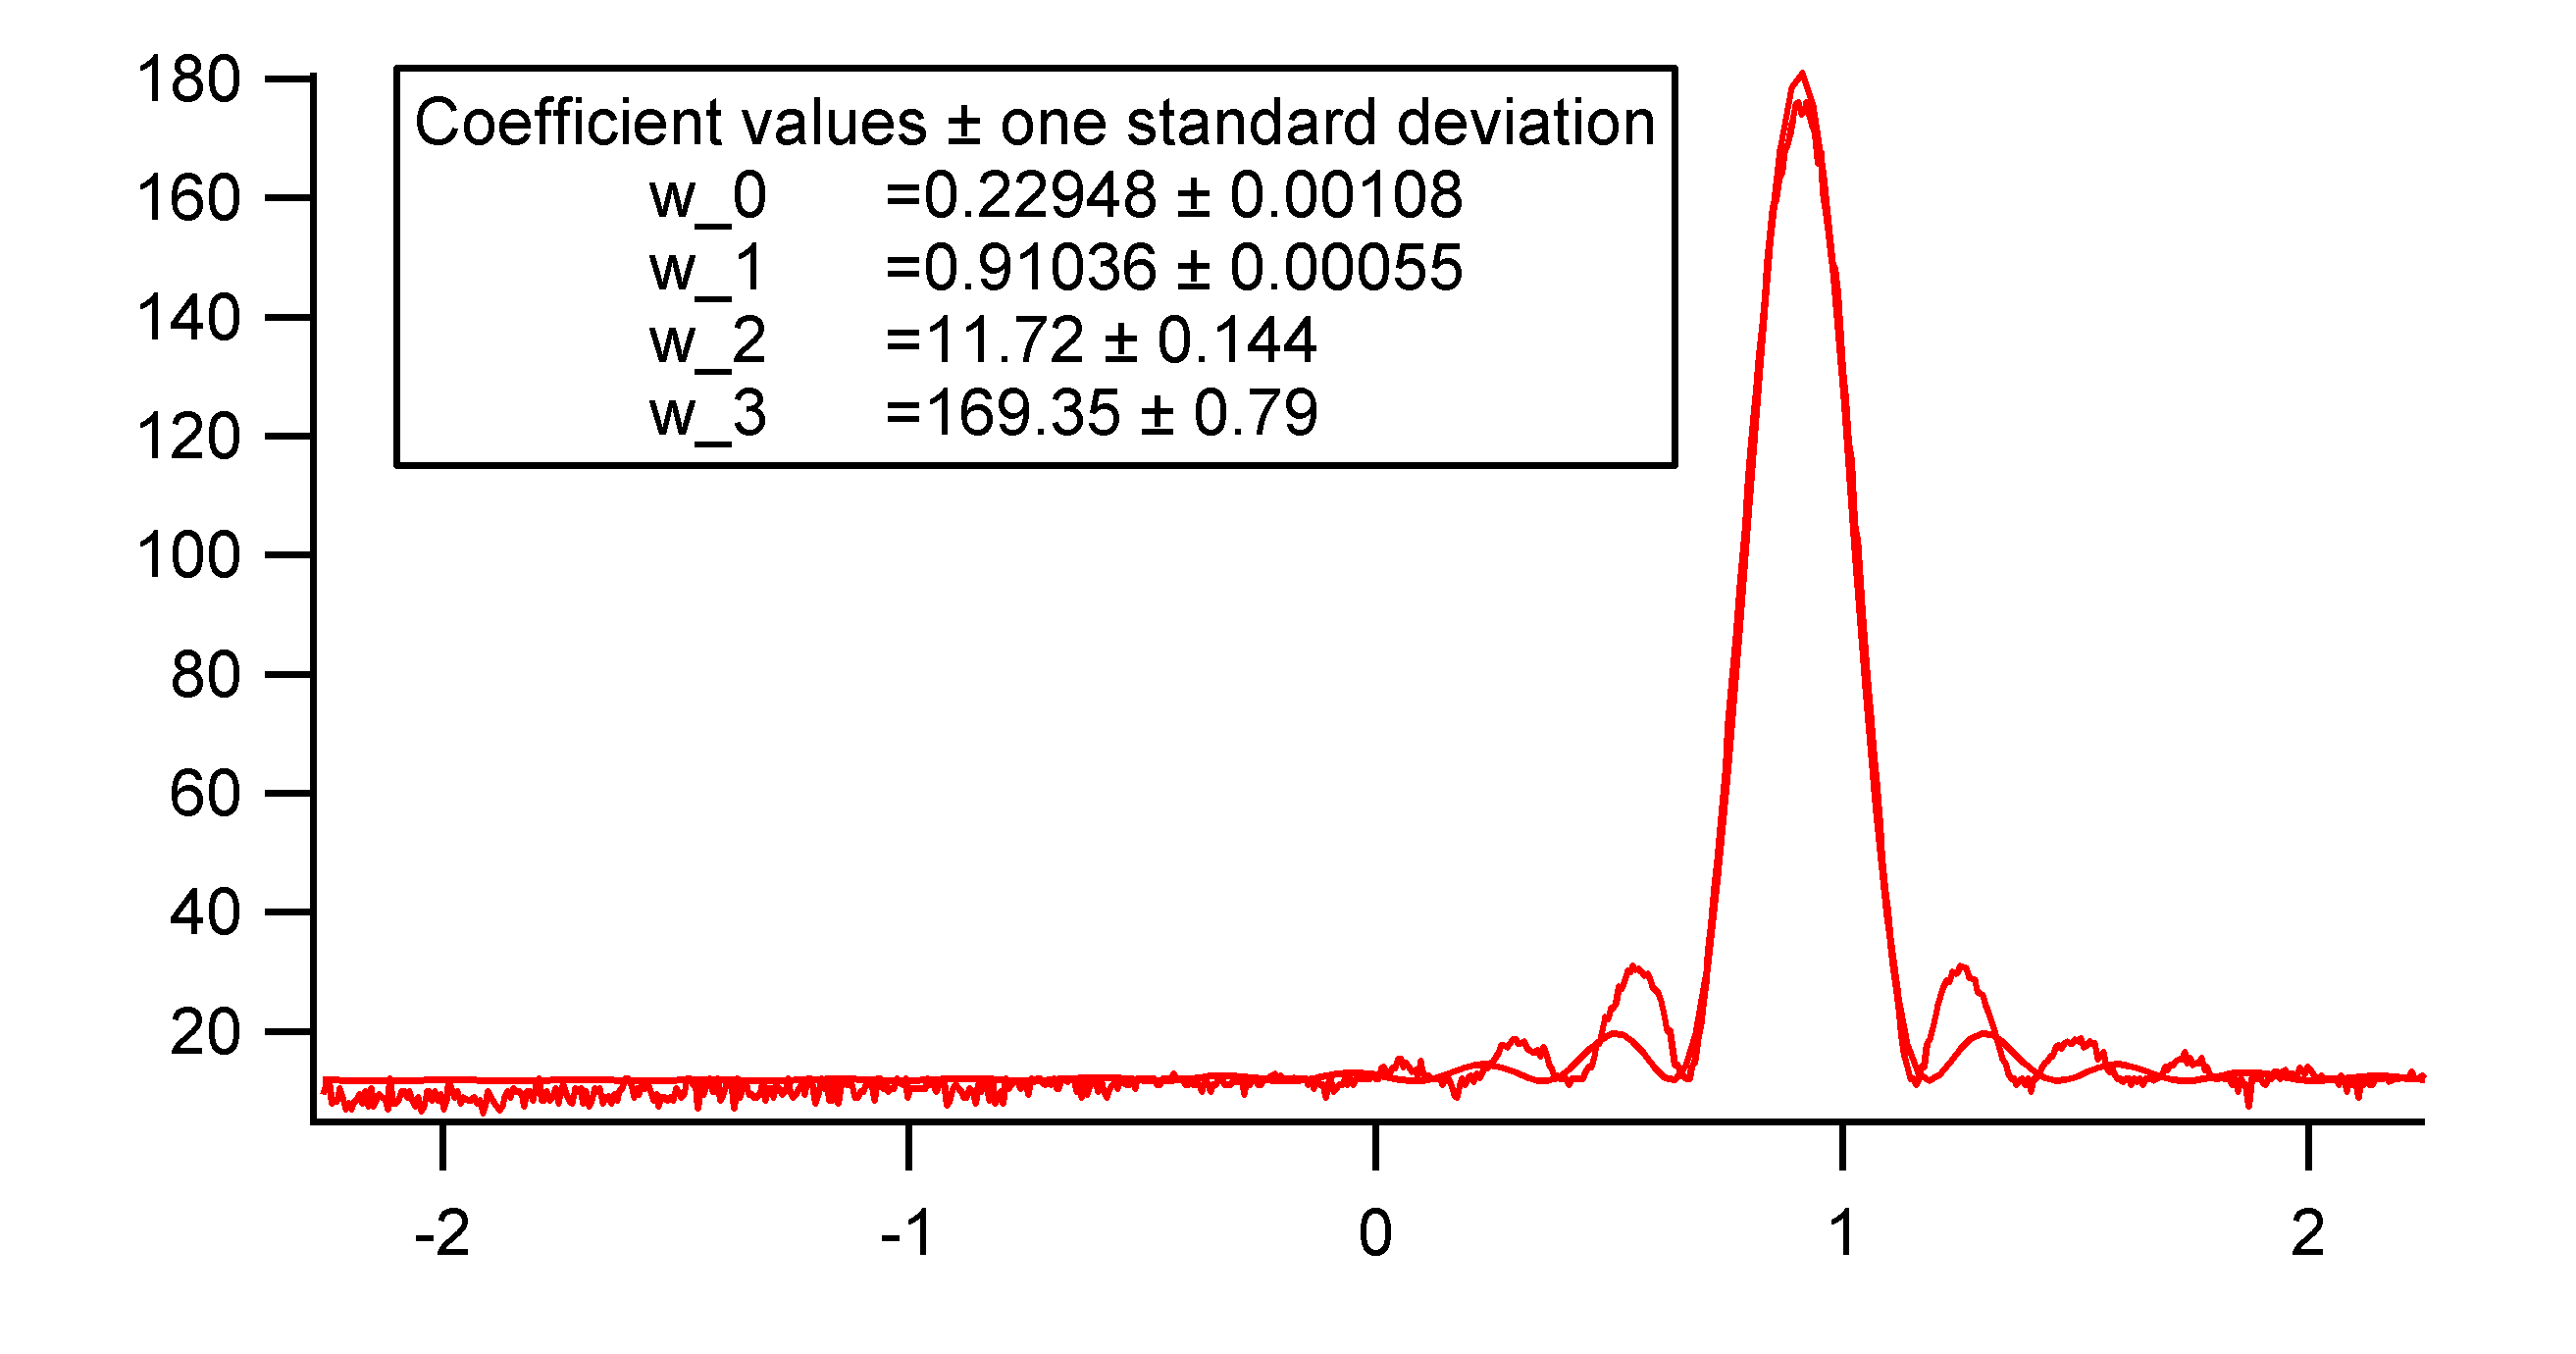
\includegraphics[width=\columnwidth]{180618/Graph2.png}
	\end{minipage}
	\caption{Beugungsmuster eines Helium-Neon-Lasers bei der Einstellung von $8~\mu m$. Der Querschnitt wurde mit Igor Pro ausgewählt und weiter analysiert }
	\label{HeNe_2}
\end{figure}
\begin{figure}[H]
	\centering	
	\begin{minipage}{1\textwidth}
		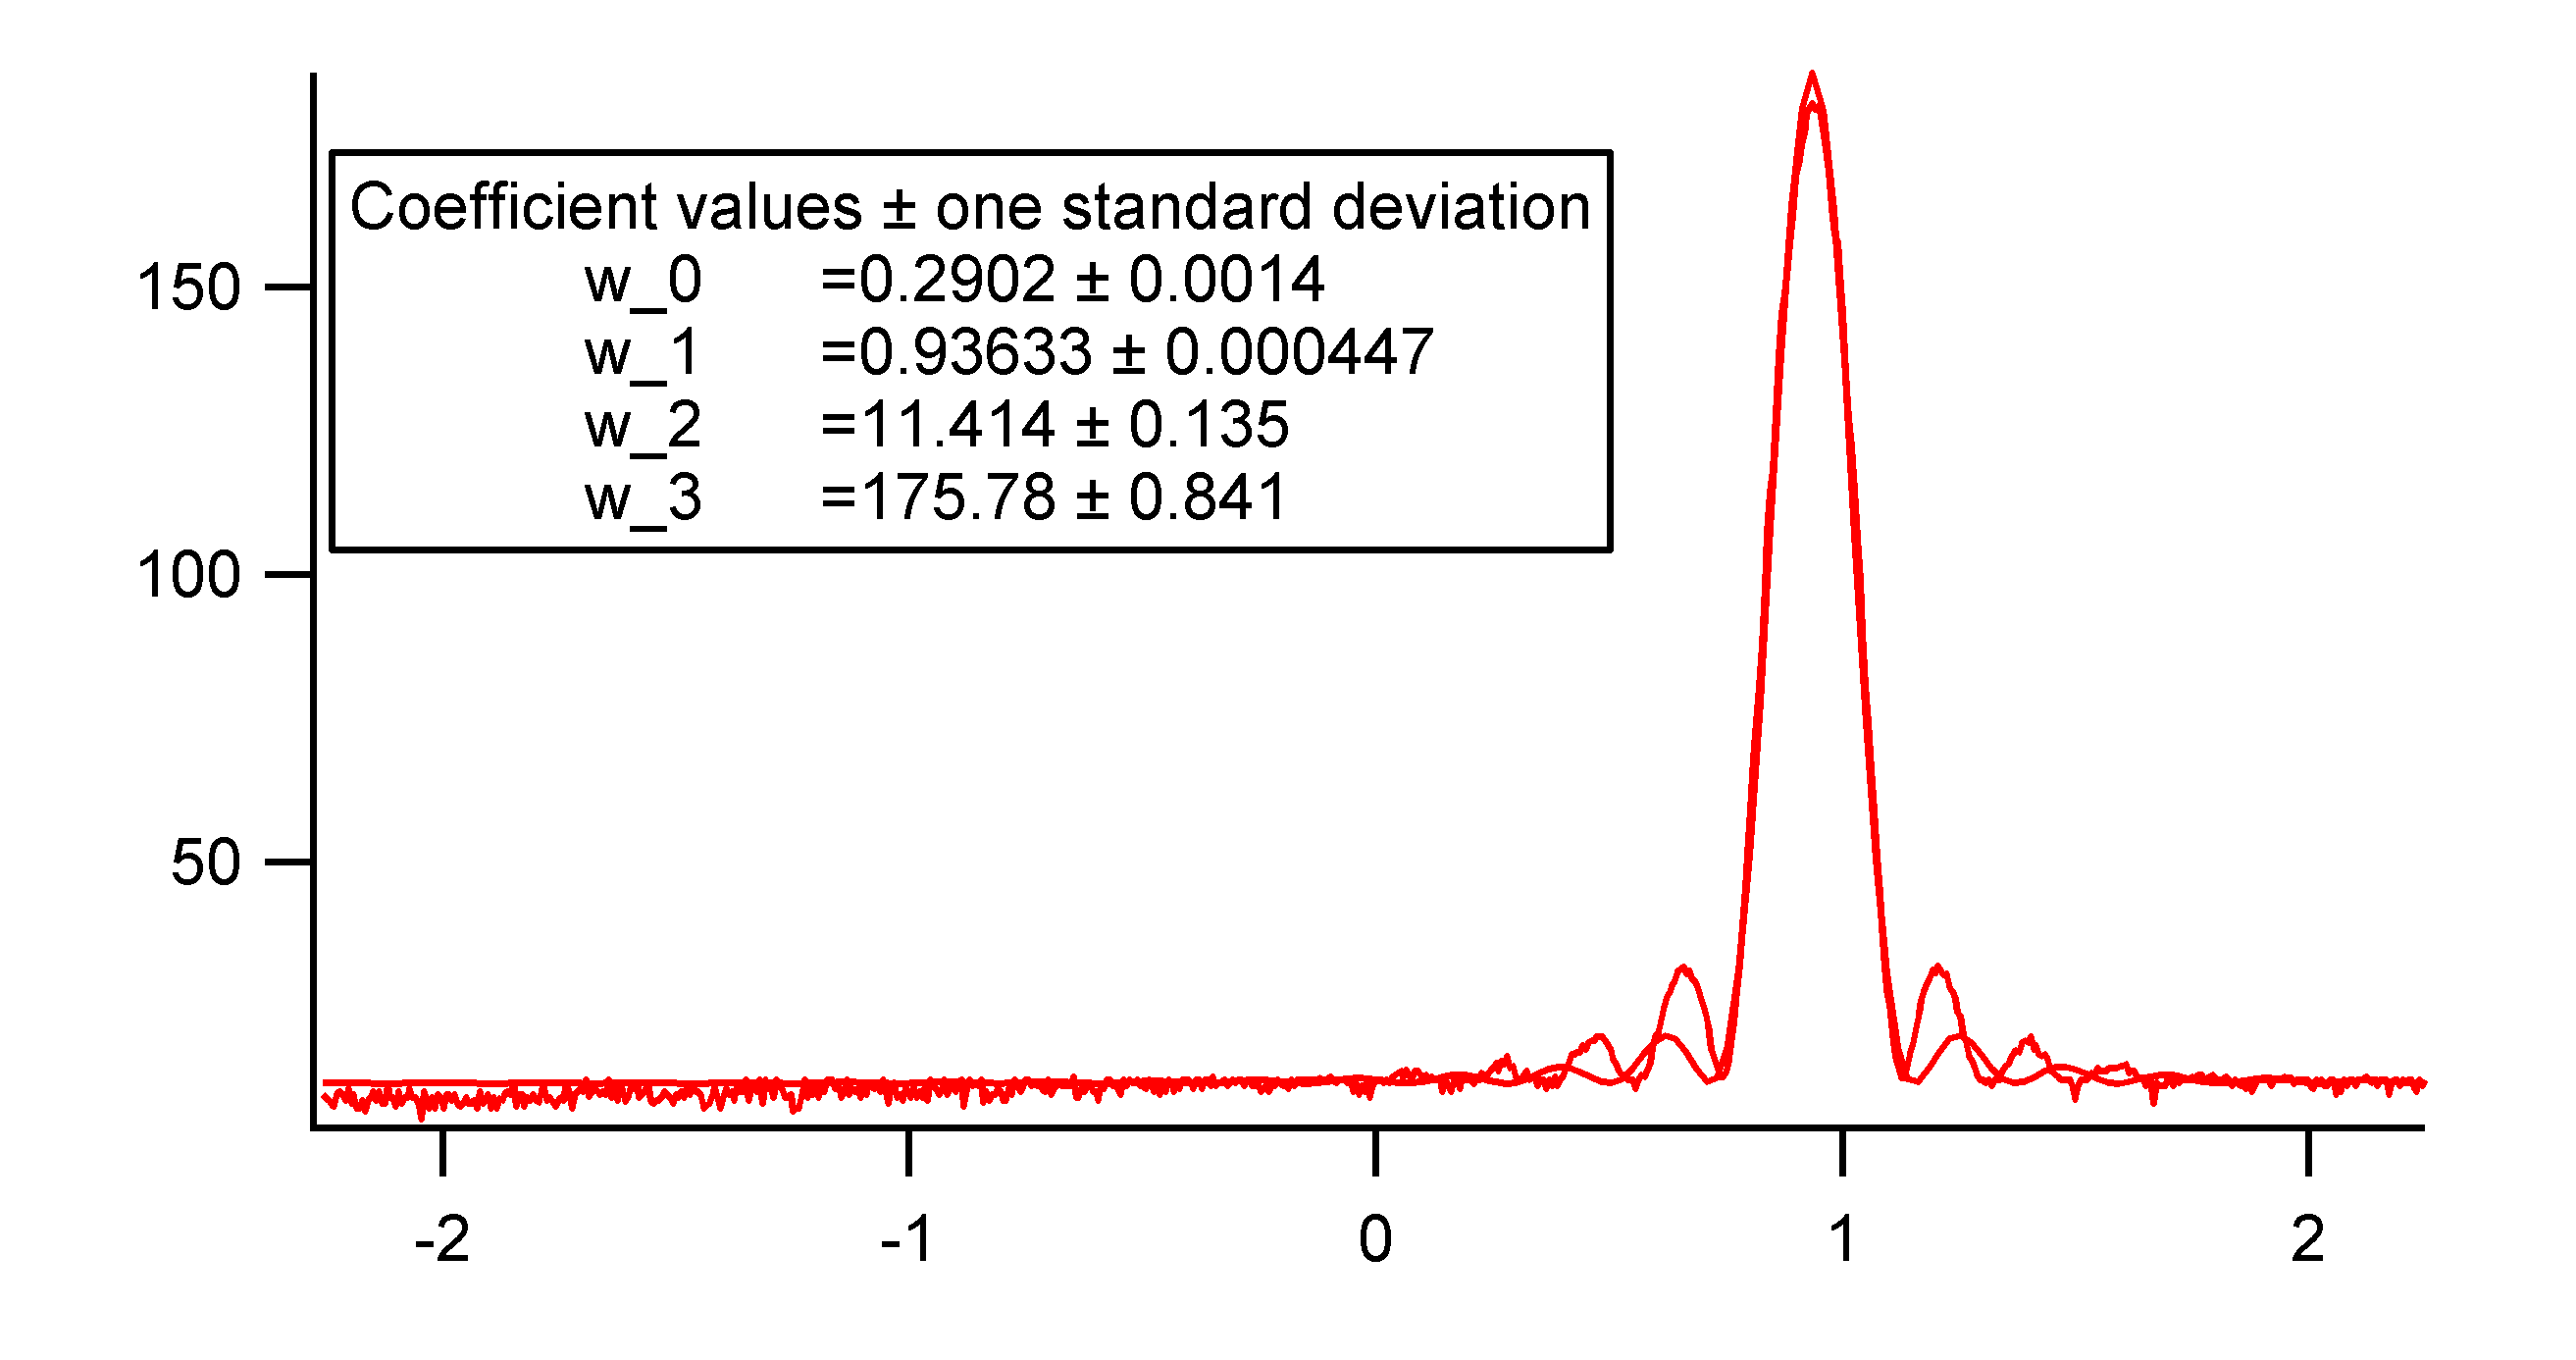
\includegraphics[width=\columnwidth]{180618/Graph3.png}
	\end{minipage}
	\caption{Beugungsmuster eines Helium-Neon-Lasers bei der Einstellung von $12~\mu m$. Der Querschnitt wurde mit Igor Pro ausgewählt und weiter analysiert }
	\label{HeNe_3}
\end{figure}
\begin{figure}[H]
	\centering	
	\begin{minipage}{1\textwidth}
		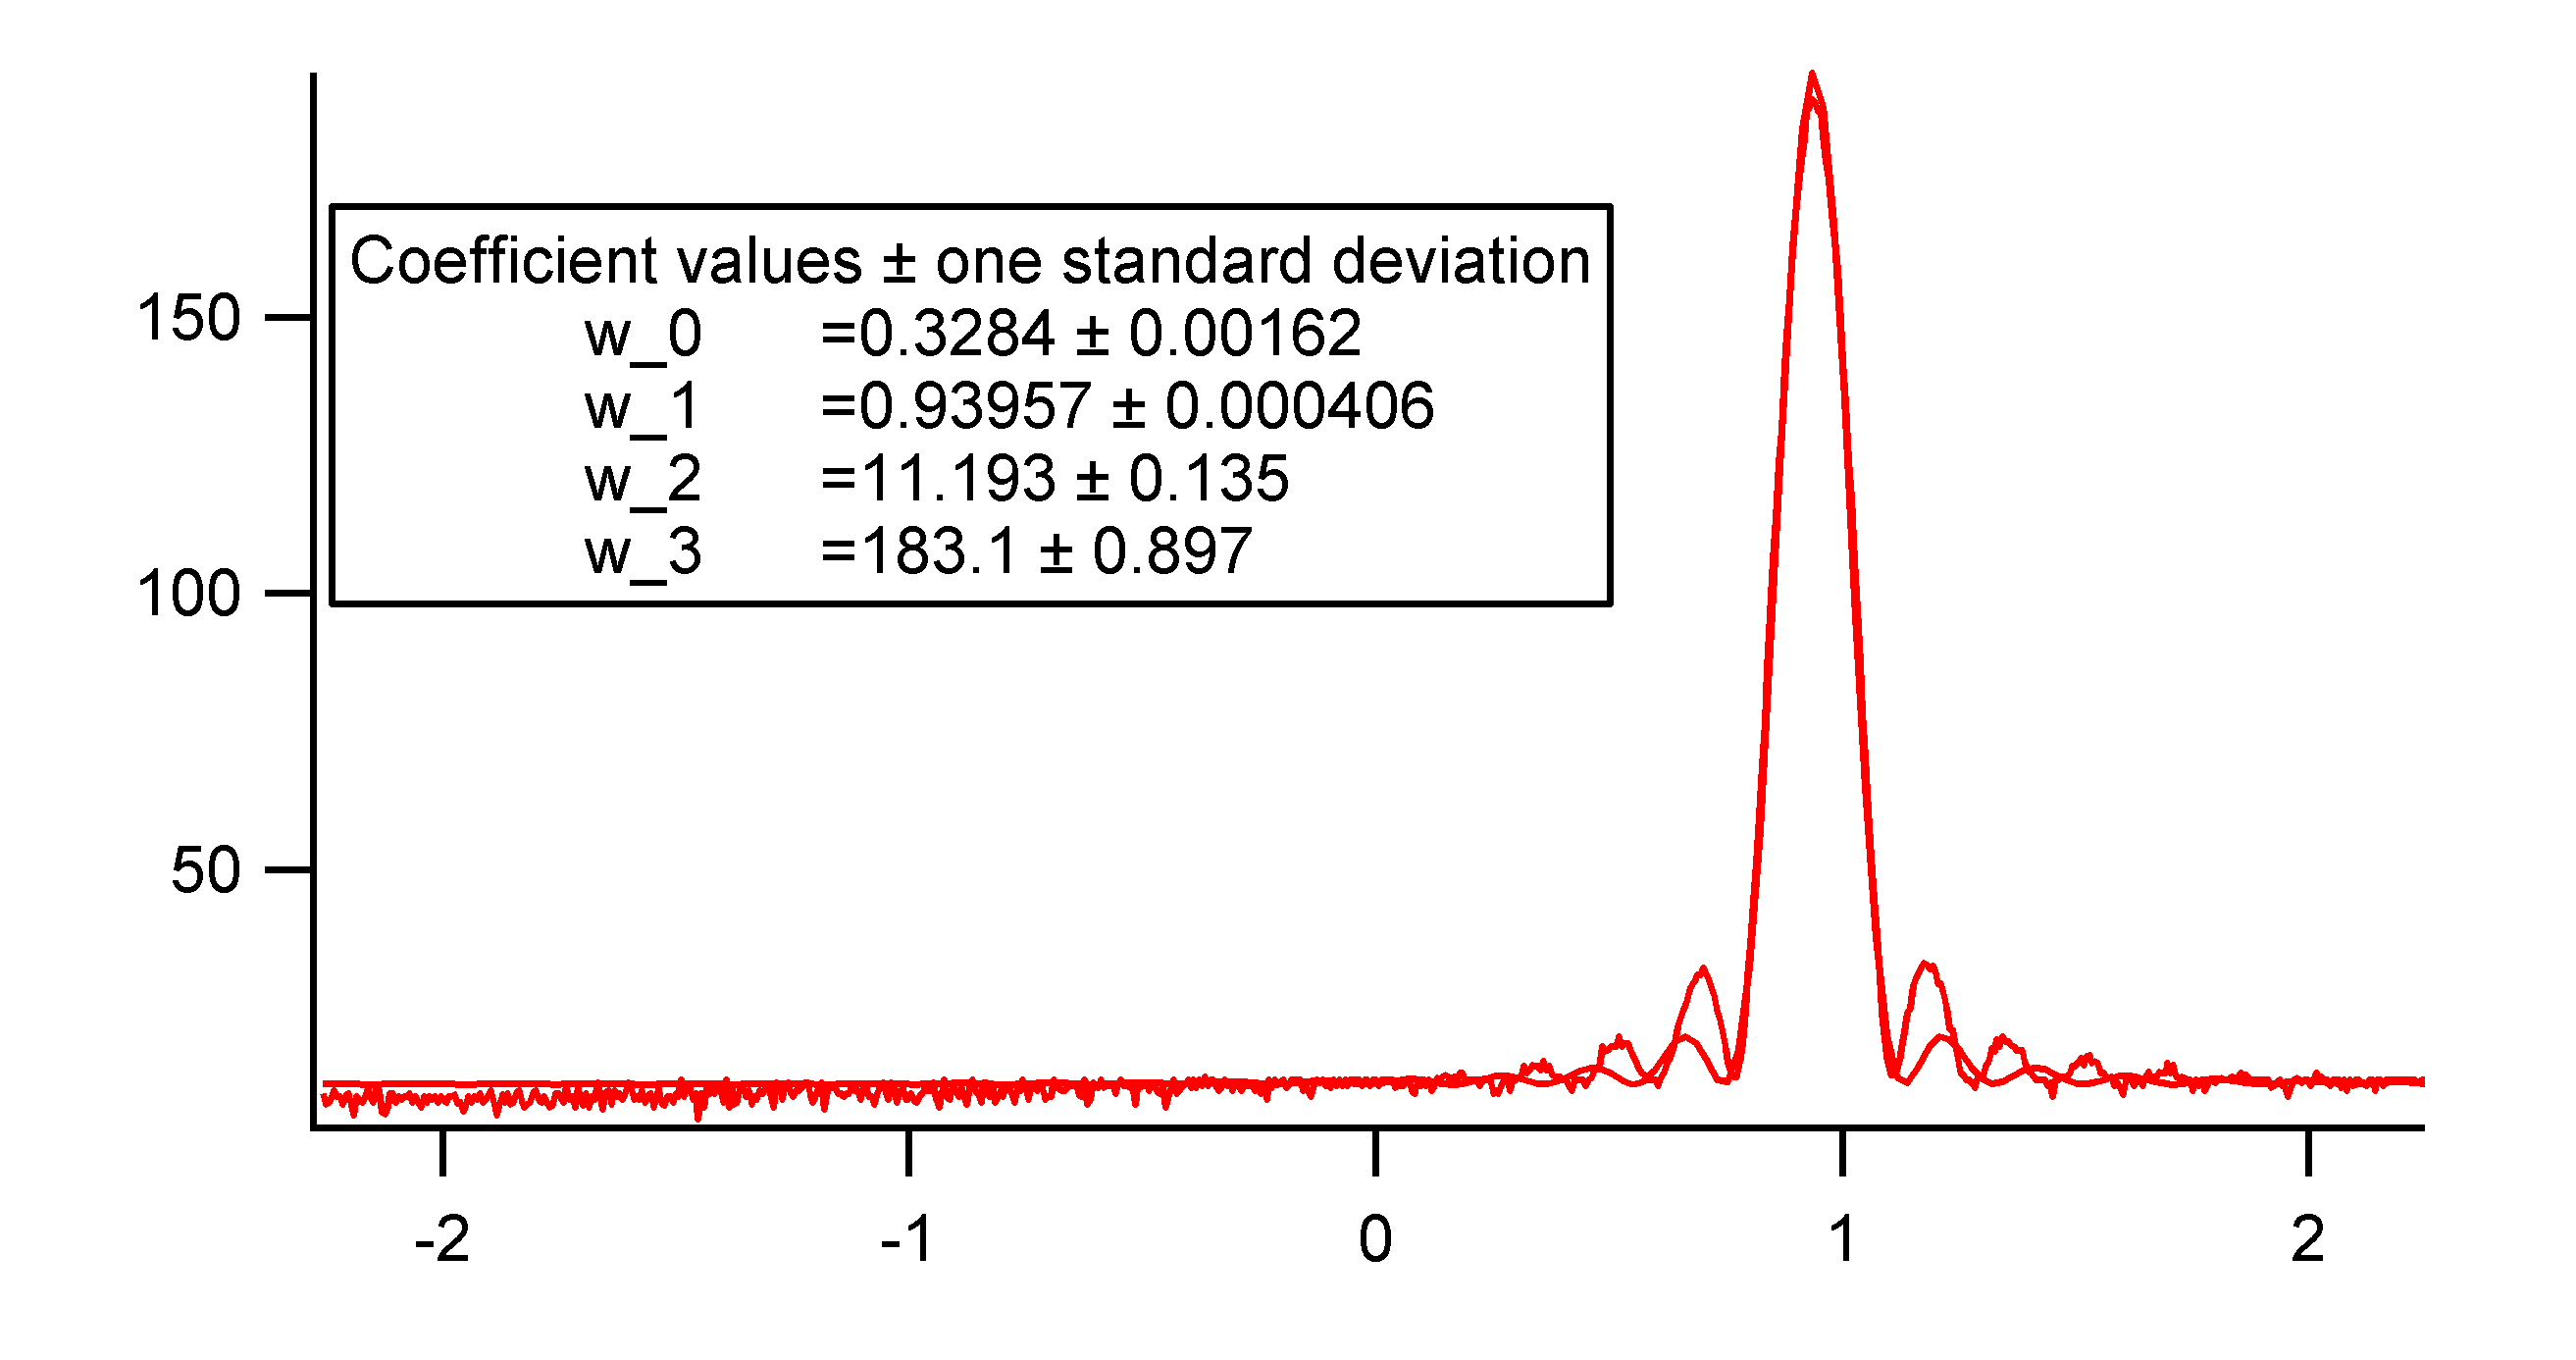
\includegraphics[width=\columnwidth]{180618/Graph4.png}
	\end{minipage}
	\caption{Beugungsmuster eines Helium-Neon-Lasers bei der Einstellung von $16~\mu m$. Der Querschnitt wurde mit Igor Pro ausgewählt und weiter analysiert }
	\label{HeNe_4}
\end{figure}
\begin{figure}[H]
	\centering	
	\begin{minipage}{1\textwidth}
		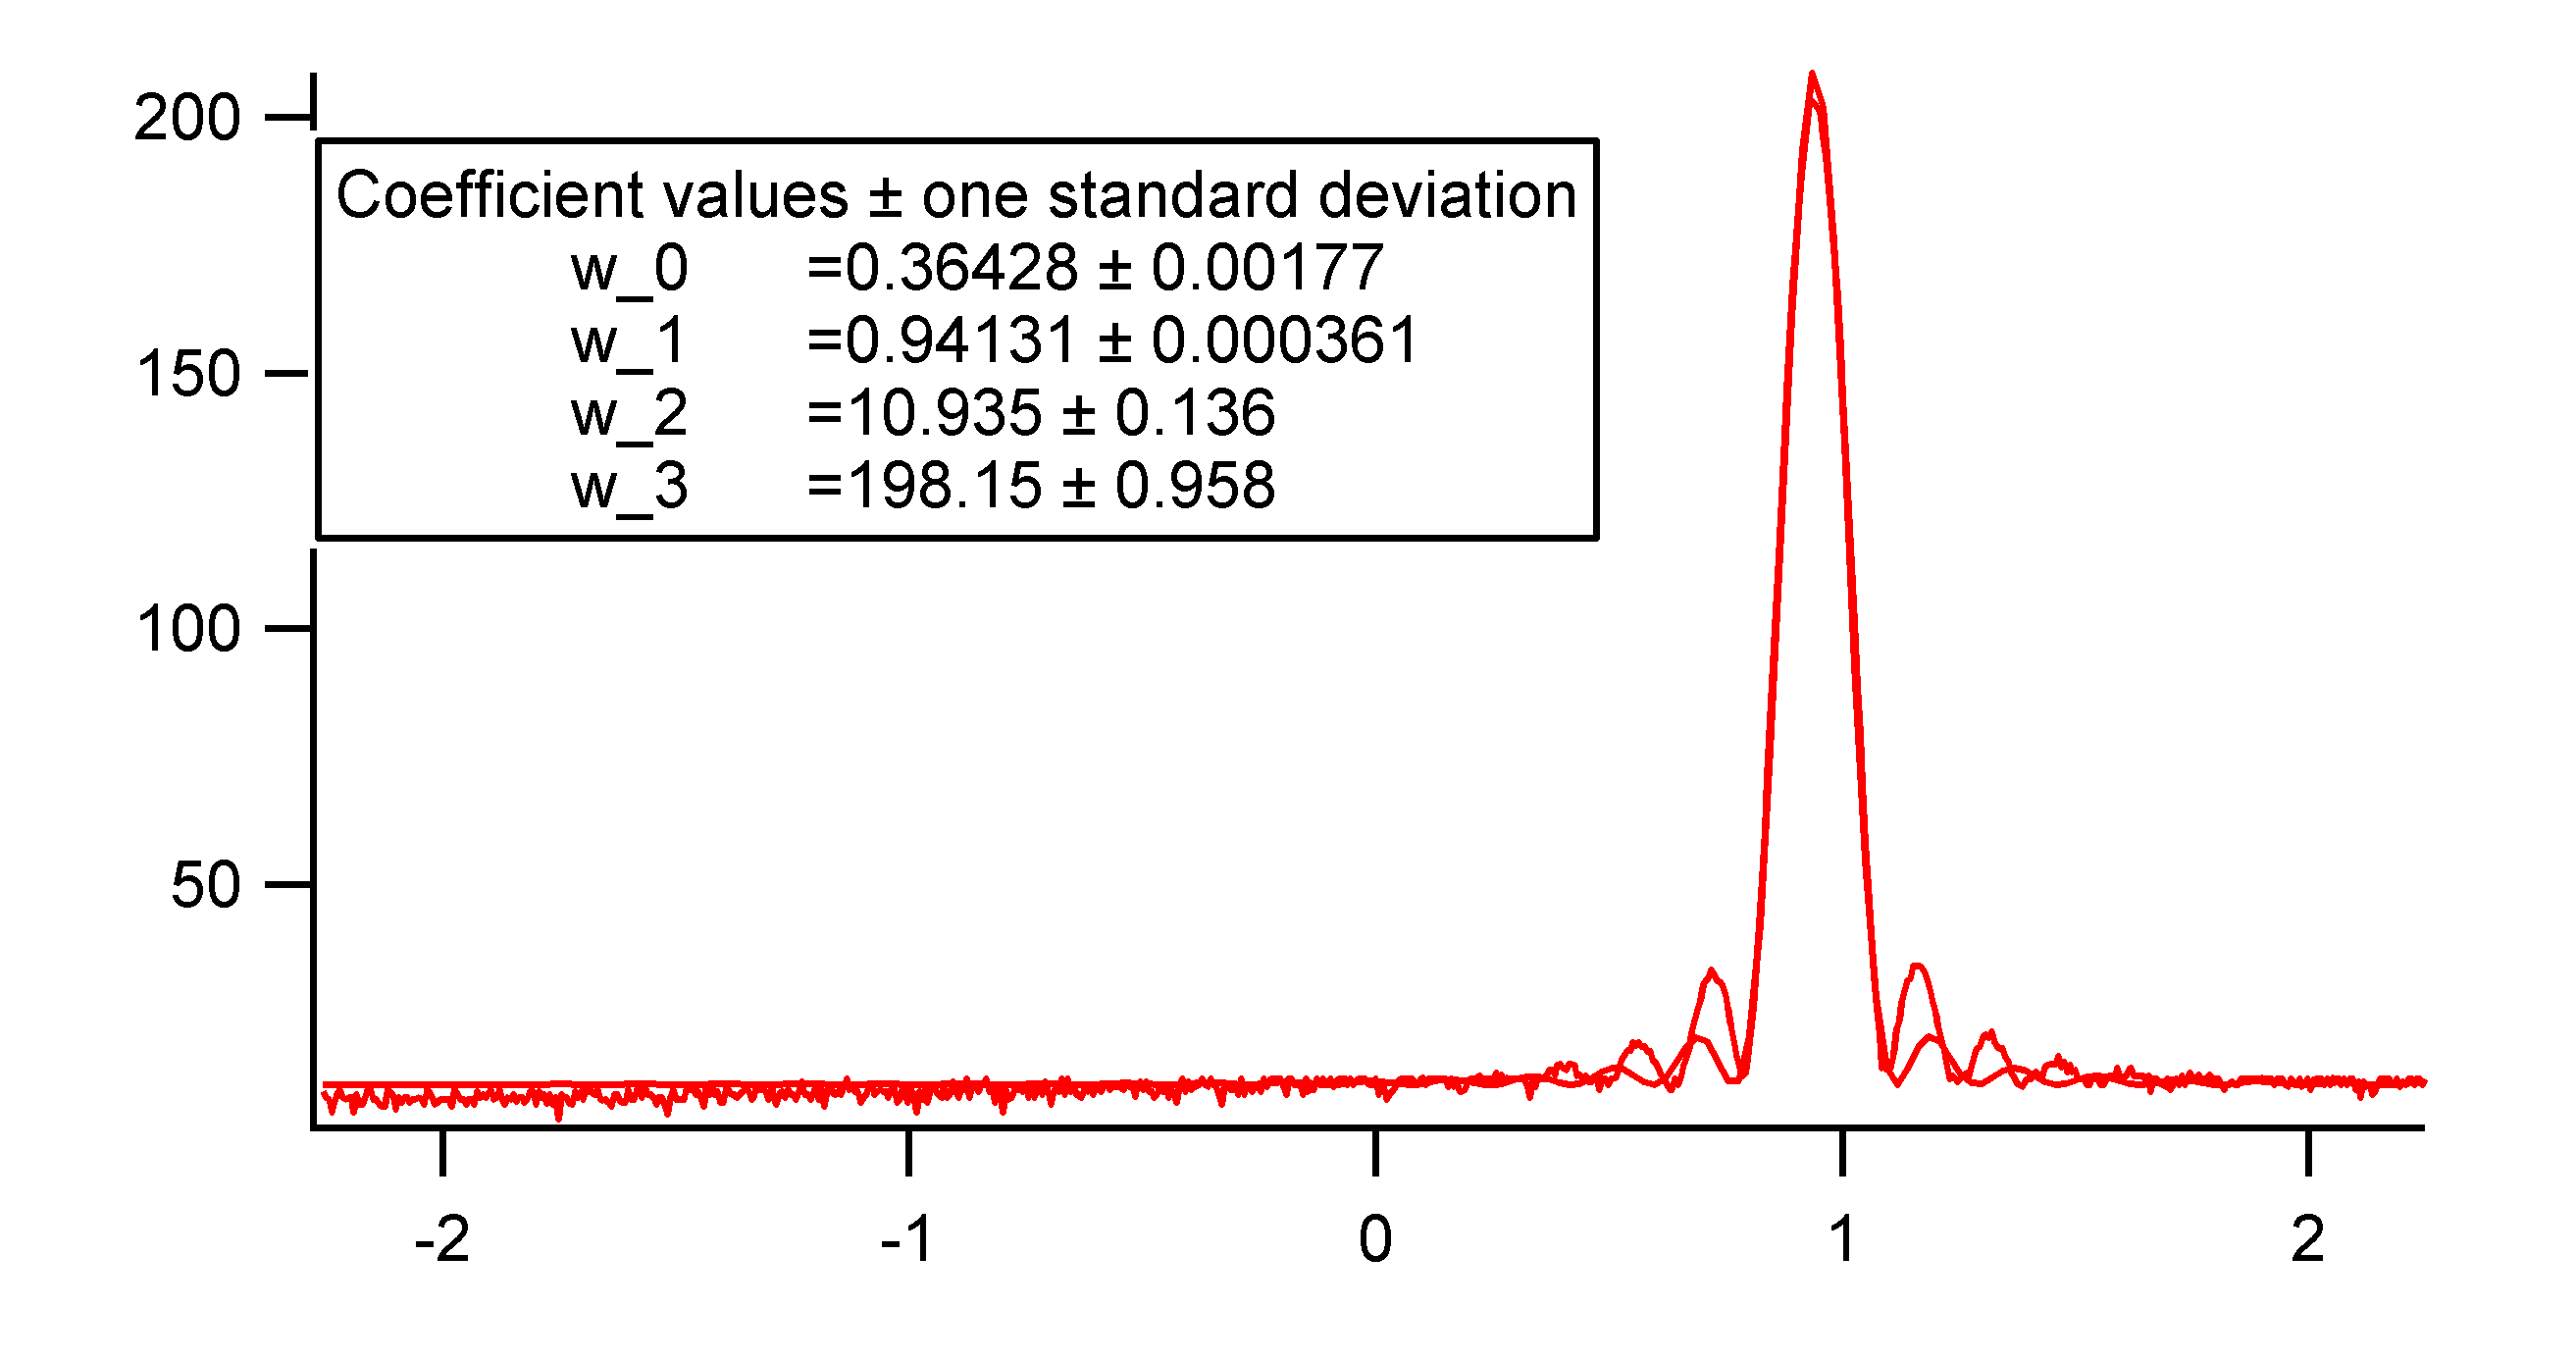
\includegraphics[width=\columnwidth]{180618/Graph5.png}
	\end{minipage}
	\caption{Beugungsmuster eines Helium-Neon-Lasers bei der Einstellung von $20~\mu m$. Der Querschnitt wurde mit Igor Pro ausgewählt und weiter analysiert }
	\label{HeNe_5}
\end{figure}
\begin{figure}[H]
	\centering	
	\begin{minipage}{1\textwidth}
		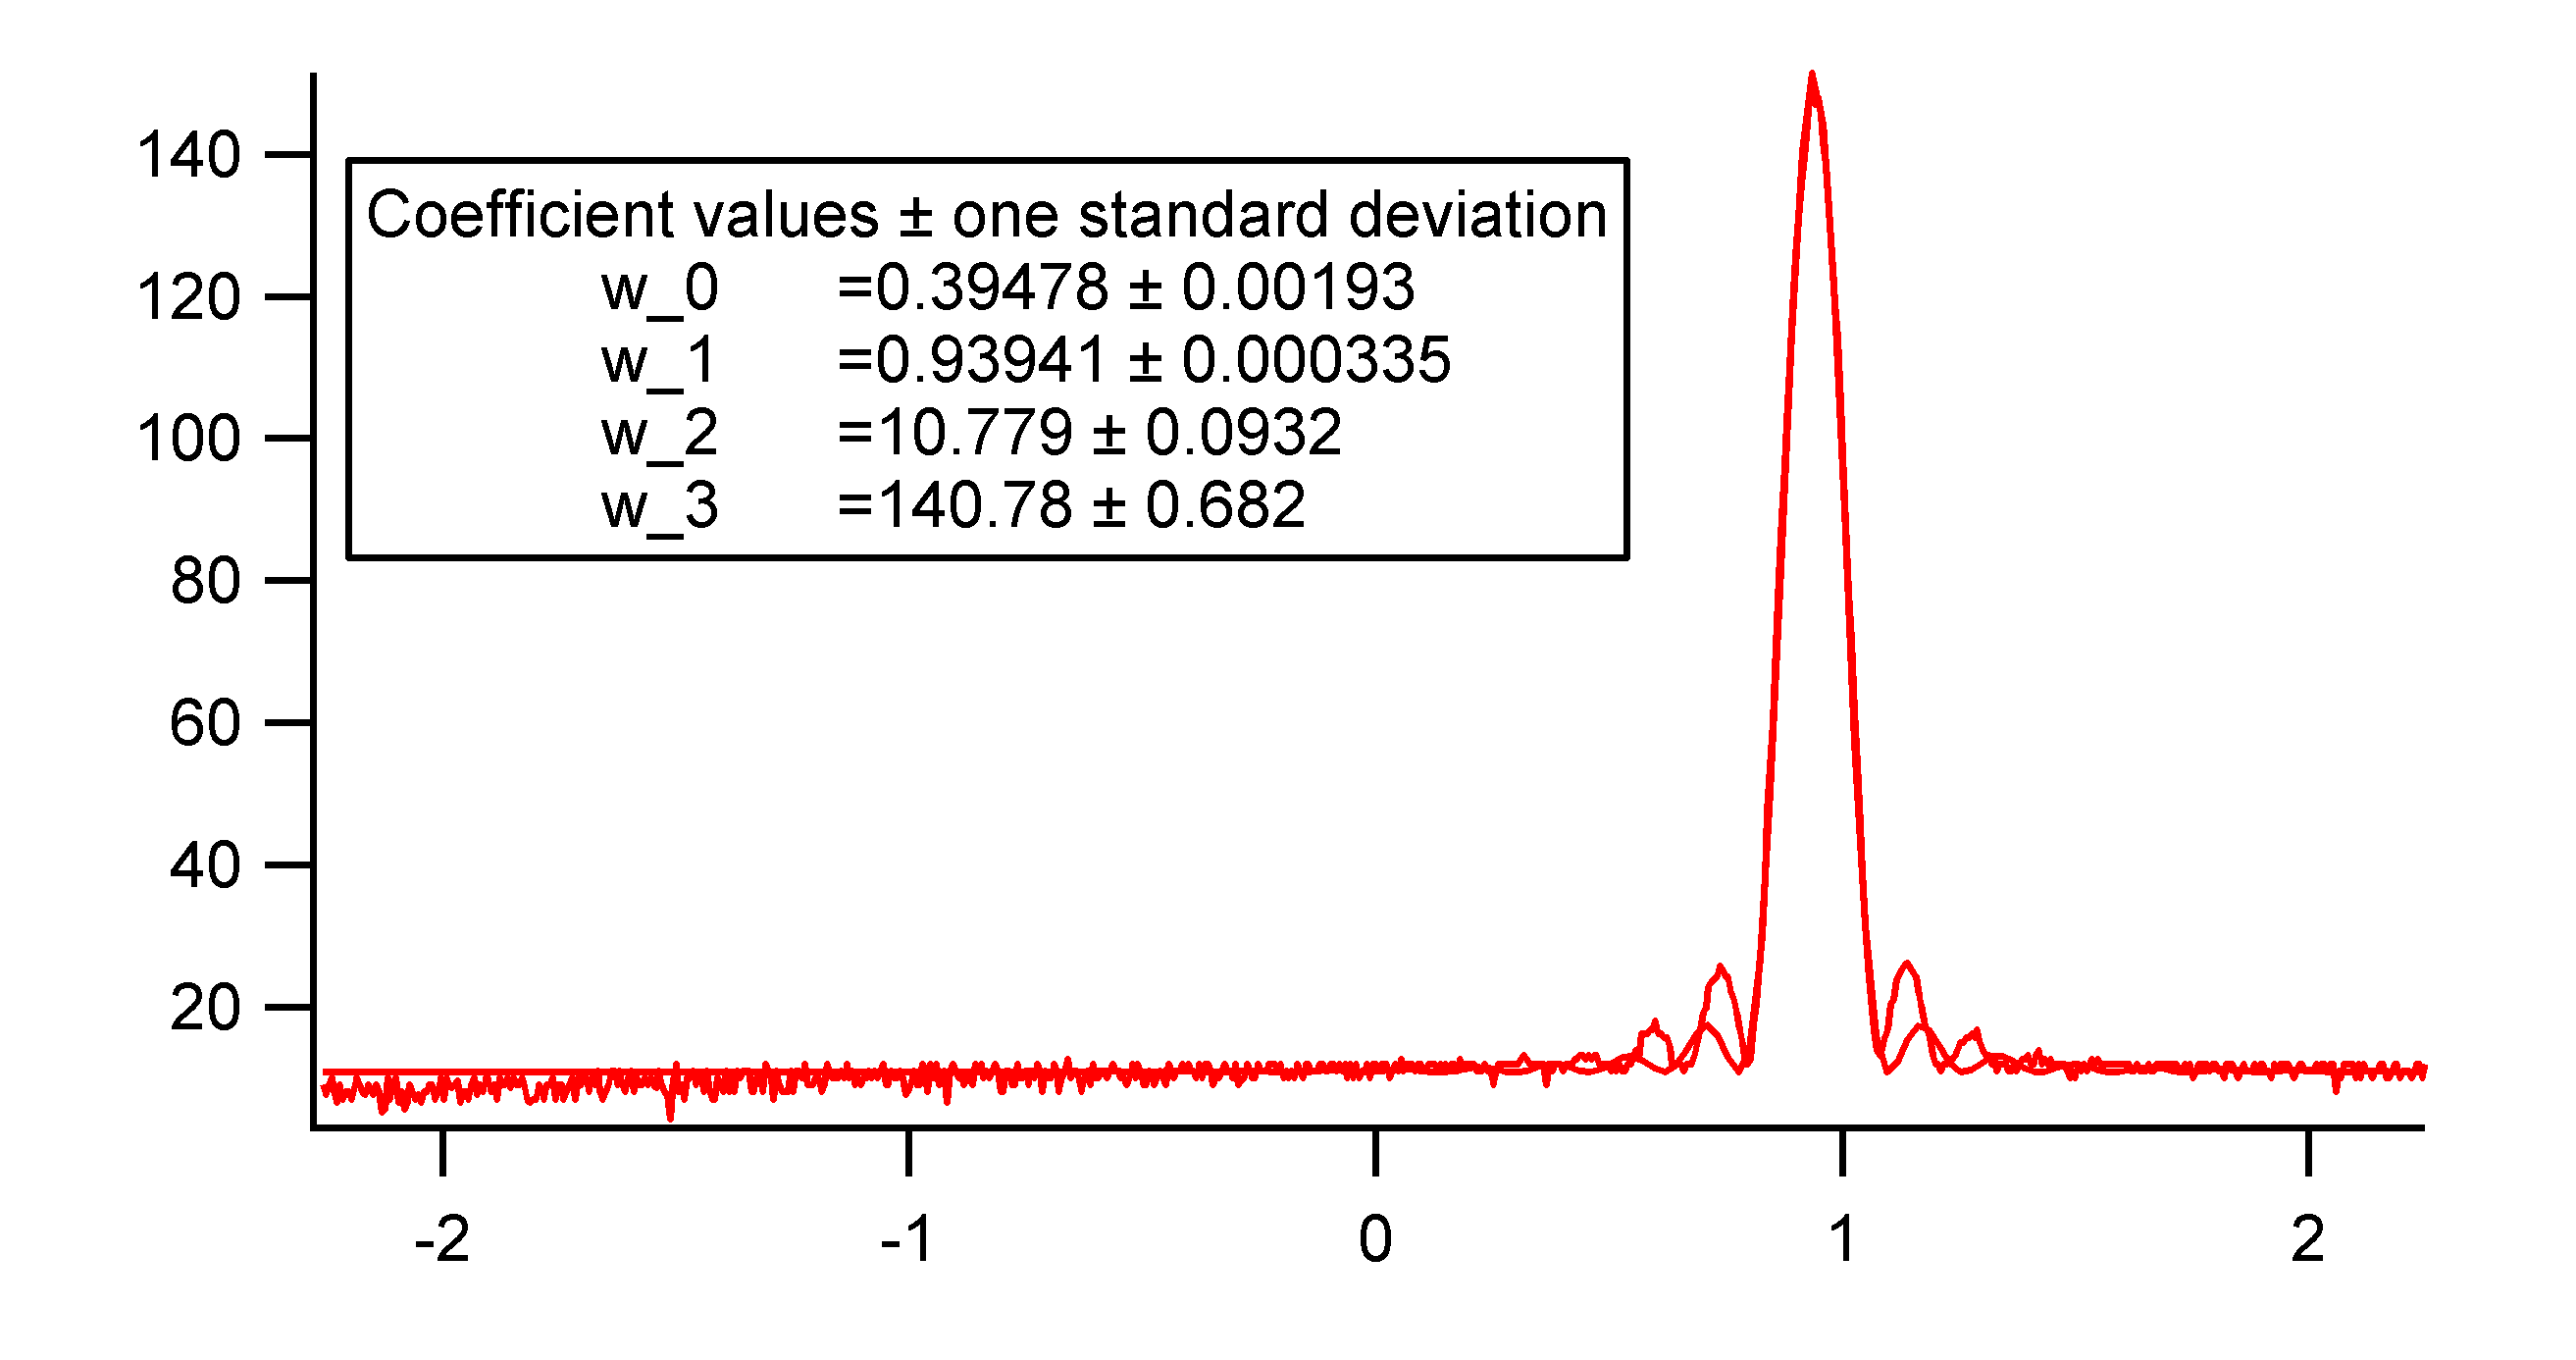
\includegraphics[width=\columnwidth]{180618/Graph6.png}
	\end{minipage}
	\caption{Beugungsmuster eines Helium-Neon-Lasers bei der Einstellung von $24~\mu m$. Der Querschnitt wurde mit Igor Pro ausgewählt und weiter analysiert }
	\label{HeNe_6}
\end{figure}





\end{document}